\documentclass{article}

% chinese fonts
\usepackage{ctex}

% math fonts
\usepackage{amsmath}
\usepackage{amsthm}
\usepackage{amssymb}
\usepackage{bm}

% figures
\usepackage{tikz}
\usepackage{graphicx}
\graphicspath{{./figures/}}

% tables
\usepackage{tabularx}
\usepackage{booktabs}
\usepackage{multirow}

% codes
\usepackage{listings}
\lstset{language     = Matlab,
        basicstyle   = \ttfamily,
        keywordstyle = \color{cyan},
        rulecolor    = \color{black},
        commentstyle = \color{green},
        keepspaces   = true,
        tabsize      = 4,
}

% hyperlinks
\usepackage{hyperref}
\hypersetup{
  breaklinks,
  colorlinks = true,
  citecolor  = blue,
  linkcolor  = red,
  urlcolor   = magenta,
}

% algorithms
\usepackage{algorithm}
\usepackage{algorithmic}

% bibliography
\usepackage[sort&compress,numbers]{natbib}

% About:  Macros for Vector, Matrix, Tensor, Math Operator and Misc
% Author: Jingxuan Yang

% vectors
\newcommand{\va}{\bm{a}}       \newcommand{\vah}{\hat{\bm{a}}}        \newcommand{\ah}{\hat{a}}    \newcommand{\vat}{\tilde{\bm{a}}}       \newcommand{\at}{\tilde{a}}
\newcommand{\vb}{\bm{b}}       \newcommand{\vbh}{\hat{\bm{b}}}        \newcommand{\bh}{\hat{b}}    \newcommand{\vbt}{\tilde{\bm{b}}}       \newcommand{\bt}{\tilde{b}}
\newcommand{\vc}{\bm{c}}       \newcommand{\vch}{\hat{\bm{c}}}        \newcommand{\ch}{\hat{c}}    \newcommand{\vct}{\tilde{\bm{c}}}       \newcommand{\ct}{\tilde{c}}
\newcommand{\vd}{\bm{d}}       \newcommand{\vdh}{\hat{\bm{d}}}        \newcommand{\dhat}{\hat{d}}  \newcommand{\vdt}{\tilde{\bm{d}}}       \newcommand{\dt}{\tilde{d}}
\newcommand{\ve}{\bm{e}}       \newcommand{\veh}{\hat{\bm{e}}}        \newcommand{\eh}{\hat{e}}    \newcommand{\vet}{\tilde{\bm{e}}}       \newcommand{\et}{\tilde{e}}
\newcommand{\vf}{\bm{f}}       \newcommand{\vfh}{\hat{\bm{f}}}        \newcommand{\fh}{\hat{f}}    \newcommand{\vft}{\tilde{\bm{f}}}       \newcommand{\ft}{\tilde{f}}
\newcommand{\vg}{\bm{g}}       \newcommand{\vgh}{\hat{\bm{g}}}        \newcommand{\gh}{\hat{g}}    \newcommand{\vgt}{\tilde{\bm{g}}}       \newcommand{\gt}{\tilde{g}}
\newcommand{\vh}{\bm{h}}     \newcommand{\vhh}{\hat{\bm{h}}}        \newcommand{\hh}{\hat{h}}    \newcommand{\vht}{\tilde{\bm{h}}}       \newcommand{\htild}{\tilde{h}}
\newcommand{\vi}{\bm{i}}       \newcommand{\vih}{\hat{\bm{i}}}        \newcommand{\ih}{\hat{i}}    \newcommand{\vit}{\tilde{\bm{i}}}       \newcommand{\itild}{\tilde{i}}
\newcommand{\vj}{\bm{j}}       \newcommand{\vjh}{\hat{\bm{j}}}        \newcommand{\jh}{\hat{j}}    \newcommand{\vjt}{\tilde{\bm{j}}}       \newcommand{\jt}{\tilde{j}}
\newcommand{\vk}{\bm{k}}       \newcommand{\vkh}{\hat{\bm{k}}}        \newcommand{\kh}{\hat{k}}    \newcommand{\vkt}{\tilde{\bm{k}}}       \newcommand{\kt}{\tilde{k}}
\newcommand{\vl}{\bm{l}}       \newcommand{\vlh}{\hat{\bm{l}}}        \newcommand{\lh}{\hat{l}}    \newcommand{\vlt}{\tilde{\bm{l}}}       \newcommand{\lt}{\tilde{l}}
\newcommand{\vm}{\bm{m}}       \newcommand{\vmh}{\hat{\bm{m}}}        \newcommand{\mh}{\hat{m}}    \newcommand{\vmt}{\tilde{\bm{m}}}       \newcommand{\mt}{\tilde{m}}
\newcommand{\vn}{\bm{n}}       \newcommand{\vnh}{\hat{\bm{n}}}        \newcommand{\nh}{\hat{n}}    \newcommand{\vnt}{\tilde{\bm{n}}}       \newcommand{\nt}{\tilde{n}}
\newcommand{\vo}{\bm{o}}       \newcommand{\voh}{\hat{\bm{o}}}        \newcommand{\oh}{\hat{o}}    \newcommand{\vot}{\tilde{\bm{o}}}       \newcommand{\ot}{\tilde{o}}
\newcommand{\vp}{\bm{p}}       \newcommand{\vph}{\hat{\bm{p}}}        \newcommand{\ph}{\hat{p}}    \newcommand{\vpt}{\tilde{\bm{p}}}       \newcommand{\pt}{\tilde{p}}
\newcommand{\vq}{\bm{q}}       \newcommand{\vqh}{\hat{\bm{q}}}        \newcommand{\qh}{\hat{q}}    \newcommand{\vqt}{\tilde{\bm{q}}}       \newcommand{\qt}{\tilde{q}}
\newcommand{\vr}{\bm{r}}       \newcommand{\vrh}{\hat{\bm{r}}}        \newcommand{\rh}{\hat{r}}    \newcommand{\vrt}{\tilde{\bm{r}}}       \newcommand{\rt}{\tilde{r}}
\newcommand{\vs}{\bm{s}}       \newcommand{\vsh}{\hat{\bm{s}}}        \newcommand{\sh}{\hat{s}}    \newcommand{\vst}{\tilde{\bm{s}}}       \newcommand{\st}{\tilde{s}}
\newcommand{\vt}{\bm{t}}       \newcommand{\vth}{\hat{\bm{t}}}        \newcommand{\that}{\hat{t}}  \newcommand{\vtt}{\tilde{\bm{t}}}       \newcommand{\ttil}{\tilde{t}}
\newcommand{\vu}{\bm{u}}       \newcommand{\vuh}{\hat{\bm{u}}}        \newcommand{\uh}{\hat{u}}    \newcommand{\vut}{\tilde{\bm{u}}}       \newcommand{\ut}{\tilde{u}}
\newcommand{\vv}{\bm{v}}       \newcommand{\vvh}{\hat{\bm{v}}}        \newcommand{\vhat}{\hat{v}}    \newcommand{\vvt}{\tilde{\bm{v}}}       \newcommand{\vtild}{\tilde{v}}
\newcommand{\vw}{\bm{w}}       \newcommand{\vwh}{\hat{\bm{w}}}        \newcommand{\wh}{\hat{w}}    \newcommand{\vwt}{\tilde{\bm{w}}}       \newcommand{\wt}{\tilde{w}}
\newcommand{\vx}{\bm{x}}       \newcommand{\vxh}{\hat{\bm{x}}}        \newcommand{\xh}{\hat{x}}    \newcommand{\vxt}{\tilde{\bm{x}}}       \newcommand{\xt}{\tilde{x}}
\newcommand{\vy}{\bm{y}}       \newcommand{\vyh}{\hat{\bm{y}}}        \newcommand{\yh}{\hat{y}}    \newcommand{\vyt}{\tilde{\bm{y}}}       \newcommand{\yt}{\tilde{y}}
\newcommand{\vz}{\bm{z}}       \newcommand{\vzh}{\hat{\bm{z}}}        \newcommand{\zh}{\hat{z}}    \newcommand{\vzt}{\tilde{\bm{z}}}       \newcommand{\zt}{\tilde{z}}

\newcommand{\valpha}{\bm{\alpha}}
\newcommand{\vbeta}{\bm{\beta}}
\newcommand{\vgamma}{\bm{\gamma}}
\newcommand{\vtheta}{\bm{\theta}}
\newcommand{\vlambda}{\bm{\lambda}}
\newcommand{\vmu}{\bm{\mu}}
\newcommand{\vomega}{\bm{\omega}}

\newcommand{\mSigma}{\bm{\Sigma}}

\newcommand{\Fc}{\mathcal{F}}
\newcommand{\Xc}{\mathcal{X}}
\newcommand{\Yc}{\mathcal{Y}}
\newcommand{\Zc}{\mathcal{Z}}
\newcommand{\Gc}{\mathcal{G}}
\newcommand{\Hc}{\mathcal{H}}
\newcommand{\Dc}{\mathcal{D}}
\newcommand{\Cc}{\mathcal{C}}
\newcommand{\Rc}{\mathcal{R}}

% matrices
\newcommand{\ma}{\bm{A}}
\newcommand{\mb}{\bm{B}}
\newcommand{\md}{\bm{D}}
\newcommand{\mH}{\bm{H}}
\newcommand{\mE}{\bm{E}}
\newcommand{\mi}{\bm{I}}
\newcommand{\mk}{\bm{K}}
\newcommand{\ml}{\bm{L}}
\newcommand{\mn}{\bm{N}}
\newcommand{\mP}{\bm{P}}
\newcommand{\mq}{\bm{Q}}
\newcommand{\mr}{\bm{R}}
\newcommand{\mU}{\bm{u}}
\newcommand{\mv}{\bm{v}}
\newcommand{\mw}{\bm{W}}
\newcommand{\mx}{\bm{X}}
\newcommand{\my}{\bm{Y}}
\newcommand{\mz}{\bm{Z}}

% tensors
\newcommand{\tp}{\mathsf{P}}
\newcommand{\tu}{\mathsf{U}}
\newcommand{\tx}{\mathsf{X}}
\newcommand{\ty}{\mathsf{Y}}
\newcommand{\tz}{\mathsf{Z}}
\newcommand{\tw}{\mathsf{W}}
\newcommand{\tf}{\mathsf{F}}
\newcommand{\ta}{\mathsf{A}}
\renewcommand{\th}{\mathsf{H}}

% norms
\newcommand{\mynorm}[2]{\| {#1} \|_{#2}}
\newcommand{\norm}[2]{\mynorm{#1}{#2}}
\newcommand{\bignorm}[2]{\left\| {#1} \right\|_{#2}}
\newcommand{\norml}[1]{\mynorm{#1}{1}}
\newcommand{\bignorml}[1]{\bignorm{#1}{1}}
\newcommand{\infnorm}[1]{\mynorm{#1}{\infty}}
\newcommand{\biginfnorm}[1]{\bignorm{#1}{\infty}}
\newcommand{\oneinf}{\ell_{1,\infty}}
\newcommand{\onetwo}{\ell_{1,2}}
\newcommand{\oneinfnorm}[1]{\mynorm{#1}{1,\infty}}
\newcommand{\bigoneinf}[1]{\bignorm{#1}{1,\infty}}
\newcommand{\onetwonorm}[1]{\mynorm{#1}{1,2}}
\newcommand{\bigonetwo}[1]{\bignorm{#1}{1,2}}
\newcommand{\enorm}[1]{\mynorm{#1}{2}}
\newcommand{\bigenorm}[1]{\bignorm{#1}{2}}
\newcommand{\znorm}[1]{\mynorm{#1}{0}}
\newcommand{\bigznorm}[1]{\bignorm{#1}{0}}
\newcommand{\frob}[1]{\|{#1}\|_{\text{F}}}
\newcommand{\bigfrob}[1]{\bignorm{#1}{\text{F}}}
\newcommand{\grpnorm}[2]{\norm{#1}{\text{Gr}(#2)}}

% math operators
\DeclareMathOperator*{\argmin}{argmin}
\DeclareMathOperator*{\argmax}{argmax}
\DeclareMathOperator{\divg}{div}
\DeclareMathOperator{\dom}{dom}
\DeclareMathOperator{\interior}{int}
\DeclareMathOperator{\ri}{ri}
\DeclareMathOperator{\sgn}{sgn}
\DeclareMathOperator{\trace}{Tr}
\DeclareMathOperator{\diag}{diag}
\DeclareMathOperator{\rank}{rank}
\DeclareMathOperator{\range}{range}
\DeclareMathOperator{\vect}{vec}
\DeclareMathOperator{\prox}{prox}
\DeclareMathOperator{\intr}{int}
\DeclareMathOperator{\relint}{ri}

% misc
\newcommand{\gs}{\geqslant}
\newcommand{\ls}{\leqslant}
\newcommand{\set}[1]{\left\{ {#1}\right\}}

\newcommand{\defeq}{\ \stackrel{\text{def}}{=}\ }
\newcommand{\ip}[2]{\left\langle#1, #2\right\rangle}
\newcommand{\reals}{\mathbb{R}}
\newcommand{\complex}{\mathbb{C}}
\newcommand{\half}{\frac{1}{2}}

\newtheorem{theorem}{Theorem}
\newtheorem{lemma}[theorem]{Lemma}
\newtheorem{proposition}[theorem]{Proposition}
\newtheorem{remark}[theorem]{Remark}
\newtheorem{corollary}[theorem]{Corollary}
\newtheorem{definition}[theorem]{Definition}


\setlength{\oddsidemargin}{-0.25 in}
\setlength{\evensidemargin}{-0.25 in} 
\setlength{\topmargin}{-0.25in} 
\setlength{\textwidth}{7 in} 
\setlength{\textheight}{8.5 in}
\setlength{\headsep}{0.25 in} 
\setlength{\parindent}{0 in}
\setlength{\parskip}{0.1 in}

\newcommand{\homework}[5]{
  \pagestyle{myheadings} 
  \thispagestyle{plain}
  \newpage
  \setcounter{page}{1} 
  \setcounter{section}{#5} 
  \noindent
  \begin{center}
    \framebox{ 
      \vbox{
        \vspace{2mm} 
        \hbox to 6.28in { {\bf
        THU-70250043-0,~Pattern~Recognition~(Spring 2021) \hfill Homework: 10} }
        \vspace{6mm} 
        \hbox to 6.28in { {\Large \hfill #1 \hfill} }
        \vspace{6mm} 
        \hbox to 6.28in { {\it Lecturer: #2 \hfill} }
        \vspace{2mm} 
        \hbox to 6.28in { {\it \hspace{14mm} #3 \hfill} }
        \vspace{2mm} 
        \hbox to 6.28in { {\it Student: #4 \hfill} }
        \vspace{2mm} 
      } 
    }
  \end{center}
  \markboth{#1}{#1} 
  \vspace*{4mm} 
}

\begin{document}

\homework{Dimensionality Reduction}{Changshui Zhang \hspace{5mm} {\tt zcs@mail.tsinghua.edu.cn}}{Hong Zhao \hspace{16mm} {\tt vzhao@tsinghua.edu.cn}}{Jingxuan Yang \hspace{10mm} {\tt yangjx20@mails.tsinghua.edu.cn}}{8}

\section*{PCA and Eigenvectors}

1. Let $\vx_1, \vx_2, \dots, \vx_n$ denote $n$ vectors in $\reals^D$, and we know the mean vector
\begin{equation}
  \bar{\vx}=\frac{1}{n}\sum_{i=1}^n\vx_i=\bm{0}\in\reals^D.
\end{equation}

We project them into a lower dimensional space by performing a linear transformation
\begin{equation}
  \vy_i=\mw^\top\vx_i,
\end{equation}
where $\vy_i\in\reals^d$, $\mw\in\reals^{D\times d}$, and $\mw^\top\mw=\mi\in\reals^{d\times d}$.

To simplify notations, we stack $\vx_i$ column by column to make a data matrix $\mx=[\vx_1, \vx_2, \ldots, \vx_n]\in\reals^{D\times n}$, and then perform the same operation on $\vy_i$ to get $\my\in\reals^{d\times n}$. Then we can calculate the covariance matrix $\mSigma_{\mx}=\mx\mx^\top$, and $\mSigma_{\my}=\my\my^\top$. Please find the matrix $\mw$ which maximizes the trace of $\mSigma_{\my}$. This problem has a closed-form solution and thus numerical solutions will not be accepted. 

解: 待求优化问题为
\begin{equation}
  \begin{aligned}
    &\max_{\mw}~\trace(\mSigma_{\my})\\
    &~\text{s.t.}\quad\mw^\top\mw=\mi
  \end{aligned}
\end{equation}

由 $\my=\mw^\top\mx$ 可得
\begin{equation}
  \trace(\mSigma_{\my})
  =\trace(\my\my^\top)
  =\trace(\mw^\top\mx\mx^\top\mw)
  =\trace(\mw^\top\mSigma_{\mx}\mw)
\end{equation}

所以上述优化问题可写为
\begin{equation}
  \begin{aligned}
    &\max_{\mw}~\trace(\mw^\top\mSigma_{\mx}\mw)\\
    &~\text{s.t.}\quad\mw^\top\mw=\mi
  \end{aligned}
\end{equation}

记 $\mw=[\vw_1,\vw_2,\dots,\vw_d]$, $\vw_i\in\reals^D$, 则 $\mw^\top\mw=\mi$ 之约束可写为
\begin{equation}
  \vw_i^\top\vw_j=\delta_{ij},\quad\forall~i,j=1,2,\dots,d
\end{equation}
其中 $\delta_{ij}$ 是 Kronecker delta 函数. 

引入 Lagrange 乘子 $\lambda_1,\lambda_2,\dots,\lambda_d$, 并记 $\mLambda=\diag(\lambda_1,\lambda_2,\dots,\lambda_d)$, 可得 Lagrange 函数为
\begin{equation}
  \begin{aligned}
    L(\mw,\mLambda)
    &=\trace(\mw^\top\mSigma_{\mx}\mw)-\sum_{i=1}^d\lambda_i(\vw_i^\top\vw_i-1)\\
    &=\trace(\mw^\top\mSigma_{\mx}\mw)-\trace(\mLambda(\mw^\top\mw-\mi))\\
  \end{aligned}
\end{equation}

注意到 $\mSigma_{\mx}$ 为对称矩阵, 可知 Lagrange 函数对 $\mw$ 的偏导数为
\begin{equation}
  \frac{\partial L(\mw,\mLambda)}{\partial\mw}
  =2\mSigma_{\mx}\mw-2\mw\mLambda
\end{equation}

令此偏导数为 $\bm{0}$ 可得
\begin{equation}
  \mSigma_{\mx}\mw=\mw\mLambda
\end{equation}

所以, $\vw_i$ 为矩阵 $\mSigma_{\mx}$ 的特征向量, 且 $\lambda_i$ 为对应的特征值.

令 Lagrange 函数对 $\mLambda$ 的偏导数为 $\bm{0}$ 可得
\begin{equation}
  \mw^\top\mw=\mi
\end{equation}

此时
\begin{equation}
  \trace(\mw^\top\mSigma_{\mx}\mw)
  =\trace(\mw^\top\mw\mLambda)
  =\trace(\mi\mLambda)
  =\trace(\mLambda)=\sum_{i=1}^d\lambda_i
\end{equation}

则最大化 $\trace(\mSigma_{\my})=\trace(\mLambda)$ 要求取 $\lambda_1,\lambda_2,\dots,\lambda_d$ 为矩阵 $\mSigma_{\mx}$ 前 $d$ 个最大的特征值. 令 $\vwt_i$ 为 $\lambda_i$ 对应的特征向量, 由矩阵 $\mSigma_{\mx}$ 为实对称矩阵可知 $\{\vwt_1,\vwt_2,\dots,\vwt_d\}$ 互相正交, 取
\begin{equation}
  \vw_i=\frac{\vwt_i}{\|\vwt_i\|},\quad\forall~i=1,2,\dots,d
\end{equation}

则 $\mw=[\vw_1,\vw_2,\dots,\vw_d]$ 亦满足 $\mw^\top\mw=\mi$, 所以此 $\mw$ 可使得 $\trace(\mSigma_{\my})$ 达到最大.

\section*{MDS and Strain}

2. In MDS, we have the distance matrix $\md\in\reals^{n\times n}$ for $n$ data points, where $\md_{i,j}=(\vx_i-\vx_j)^\top(\vx_i-\vx_j)$. We first get the inner product matrix $\mb$ by
\begin{equation}
  \mb=-\frac{1}{2}\mH\md\mH,
\end{equation}
where $\mH$ is defined as $\mH\triangleq\mi-\frac{1}{n}\bm{1}\bm{1}^\top$, $\bm{1}=(1,1,\dots,1)^\top\in\reals^{n\times 1}$ and $\mi\in\reals^{n\times n}$ is the identity matrix.

Suppose the desired number of dimensions for output is $m$. In the next step of MDS we should find the $m$ largest eigenvalues values $\lambda_1, \lambda_2, \dots, \lambda_m$ and corresponding eigenvectors $\vu_1, \vu_2, \dots, \vu_m\in\reals^n$ of matrix $\mb$ and the final output of MDS should be $\mx=[\vu_1, \vu_2, \dots, \vu_m]\cdot\diag(\sqrt{\lambda_1}, \sqrt{\lambda_2}, \dots, \sqrt{\lambda_m})$. Please prove that this procedure is equivalent to find $\mx$ to minimize the strain, which is defined by
\begin{equation}
  \mathrm{Strain}(\vx_1,\vx_2,\dots,\vx_n)=\sqrt{\frac{\sum_{i,j}(\mb_{i,j} - \vx_i^\top\vx_j)^2}{\sum_{i,j}\mb_{i,j}}}.
\end{equation}

解: 记 $\mU=[\vu_1, \vu_2, \dots, \vu_m]$, $\mLambda=\diag(\lambda_1, \lambda_2, \dots, \lambda_m)$, 则 $\mb=\mU\mLambda\mU^\top$,  MDS 得到
\begin{equation}
  \mx
  =[\vu_1, \vu_2, \dots, \vu_m]\cdot\diag(\sqrt{\lambda_1}, \sqrt{\lambda_2}, \dots, \sqrt{\lambda_m})
  =\mU\mLambda^{\half}
\end{equation}

关于最小化 strain, 易知
\begin{equation}
  \min_{\mx\in\reals^{n\times m}}\sqrt{\frac{\sum_{i,j}(\mb_{i,j} - \vx_i^\top\vx_j)^2}{\sum_{i,j}\mb_{i,j}}}
  \Longleftrightarrow
  \min_{\mx\in\reals^{n\times m}}\sum_{i=1}^n\sum_{j=1}^n(\mb_{i,j} - \vx_i^\top\vx_j)^2
\end{equation}

由于
\begin{equation}
  (\mb_{i,j} - \vx_i^\top\vx_j)^2\gs0,\quad\forall~i,j=1,2,\dots,n
\end{equation}

则 strain 最小值为 0, 且等号能够取到当且仅当
\begin{equation}
  \mb_{i,j} - \vx_i^\top\vx_j=0,\quad\forall~i,j=1,2,\dots,n
\end{equation}

写成矩阵形式即
\begin{equation}
  \mb=\mx\mx^\top
\end{equation}

又 $\mb=\mU\mLambda\mU^\top$, 则有 $\mx=\mU\mLambda^{\half}$, 与 MDS 得到的 $\mx$ 相同, 即 MDS 由内积矩阵 $\mb$ 求取 $\mx$ 的步骤与最小化 strain 等价.

% 以下是求导解法,麻烦没有必要又得不出充要条件,故予以舍弃
% 由
% \begin{equation}
%   \mx=\begin{bmatrix}
%     \vx_1^\top \\ 
%     \vx_2^\top \\ 
%     \vdots \\ 
%     \vx_n^\top \\
%   \end{bmatrix}
% \end{equation}

% 可知 $\mx_{p,q}=\vx_p^{(q)}$, 注意到矩阵 $\mb$ 是对称矩阵, 则 $S$ 对 $\mx_{p,q}$ 的偏导数为
% \begin{equation}
%   \begin{aligned}
%     \frac{\partial S}{\partial\mx_{p,q}}
%     &=\frac{\partial S}{\partial\vx_p^{(q)}}\\
%     &=\frac{\partial}{\partial\vx_p^{(q)}}\sum_{i=1}^n\sum_{j=1}^n(\mb_{i,j} - \vx_i^\top\vx_j)^2\\
%     &=-2\sum_{j=1}^n(\mb_{p,j} - \vx_p^\top\vx_j)\vx_j^{(q)}-2\sum_{i=1}^n(\mb_{i,p} - \vx_i^\top\vx_p)\vx_i^{(q)}\\
%     &=-2\sum_{j=1}^n(\mb_{p,j} - \vx_p^\top\vx_j)\vx_j^{(q)}-2\sum_{j=1}^n(\mb_{j,p} - \vx_j^\top\vx_p)\vx_j^{(q)}\\
%     &=-4\sum_{j=1}^n(\mb_{p,j} - \vx_p^\top\vx_j)\vx_j^{(q)}\\
%     &=-4\Big[\mb_{p,\bullet}\mx_{\bullet,q}-(\mx\mx^\top)_{p,\bullet}\mx_{\bullet,q}\Big]
%   \end{aligned}
% \end{equation}

% 则 $S$ 对 $\mx$ 的偏导数为
% \begin{equation}
%   \frac{\partial S}{\partial\mx}
%   =-4(\mb\mx-\mx\mx^\top\mx)
% \end{equation}

% 令此偏导数为 $\bm{0}$ 可得
% \begin{equation}
%   \mb\mx=\mx\mx^\top\mx
% \end{equation}

% 当 $\mx=\mU\mLambda^{\half}$ 时, 有
% \begin{equation}
%   \mb\mx
%   =\mb\mU\mLambda^{\half}
%   =\mU\mLambda\mU^\top\mU\mLambda^{\half}
%   =\mU\mLambda\mLambda^{\half}
% \end{equation}

% 且
% \begin{equation}
%   \mx\mx^\top\mx
%   =\mU\mLambda^{\half}\mLambda^{\half}\mU^\top\mU\mLambda^{\half}
%   =\mU\mLambda\mLambda^{\half}
% \end{equation}

% 即 $\mb\mx=\mx\mx^\top\mx$.

\section*{ISOMAP and LLE}

\emph{ISOMAP, LLE 对流形的降维}

3. 考虑如下的问题并实现 ISOMAP, LLE 等降维方法. \emph{注意}: 数据在产生过程中可不必严格保证形状, 大致符合要求即可, 不用在数据的产生上花费过多时间. 可以参考 \href{https://scikit-learn.org/stable/auto_examples/manifold/plot_compare_methods.html\#sphx-glr-auto-examples-manifold-plot-compare-methods-py}{scikit-learn 的官方文档}, 实现类似的效果, 但是不可以直接使用已有的 LLE 和 ISOMAP 函数.

3.1. 在三维空间中产生 ``Z'' 形状的流形, 使用 ISOMAP 方法降维并作图, 给出数据的三维分布图和最佳参数下的降维效果图.

解: 生成 ``Z'' 形状的流形数据如图 \ref{fig:manifoldZ} 所示, 使用 ISOMAP 方法降维, 选择 20 近邻计算距离, 得到降维后的结果如图 \ref{fig:reducedZ} 所示, ISOMAP 将三维数据降维到二维平面, 并且保持着数据点在二维流形上的位置关系.

\begin{figure}[htbp]
  \centering
  \begin{minipage}[t]{0.48\textwidth}
    \centering
    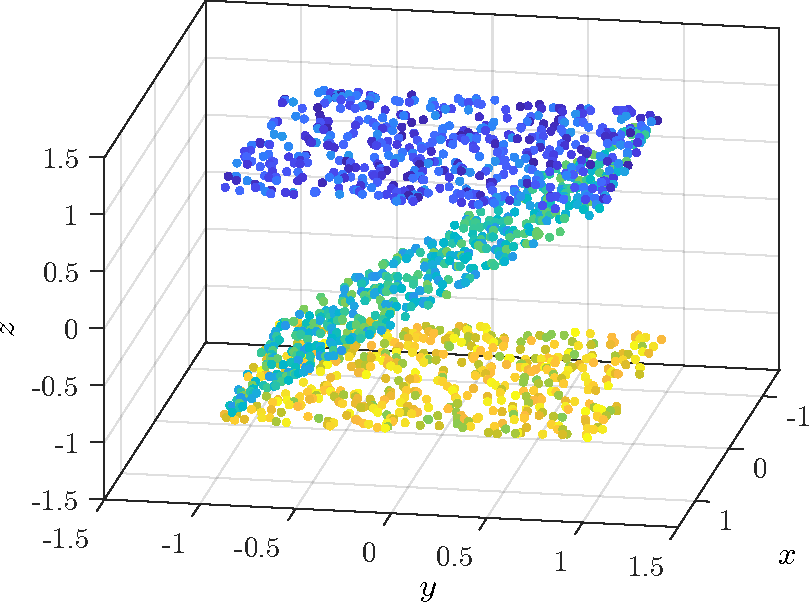
\includegraphics[width=8cm]{manifoldZ.pdf}
    \caption{``Z'' 形状流形数据分布图}
    \label{fig:manifoldZ}
  \end{minipage}
  \begin{minipage}[t]{0.48\textwidth}
    \centering
    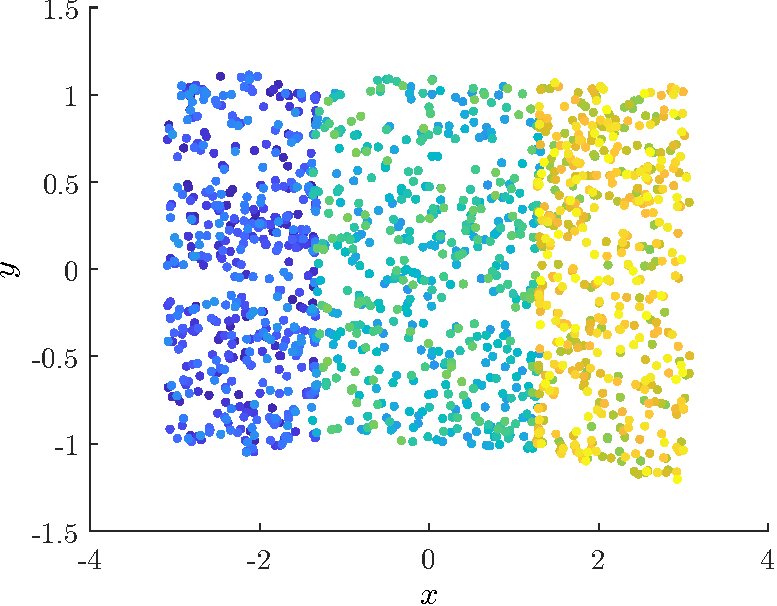
\includegraphics[width=8cm]{reducedZ.pdf}
    \caption{``Z'' 形状流形数据 ISOMAP 降维结果}
    \label{fig:reducedZ}
  \end{minipage}
\end{figure}

3.2. 在三维空间中产生 ``W'' 形状的流形, 使用 LLE 方法降维并作图, 给出数据的三维分布图和最佳参数下的降维效果图.

解: 生成 ``W'' 形状的流形数据如图 \ref{fig:manifoldW} 所示, 使用 LLE 方法降维, LLE 算法部分代码参考网站 \cite{lle}, 选择 40 近邻计算距离, 得到降维后的结果如图 \ref{fig:reducedW} 所示, LLE 将三维数据降维到二维平面, 并且保持了良好的可分性.

\begin{figure}[htbp]
  \centering
  \begin{minipage}[t]{0.48\textwidth}
    \centering
    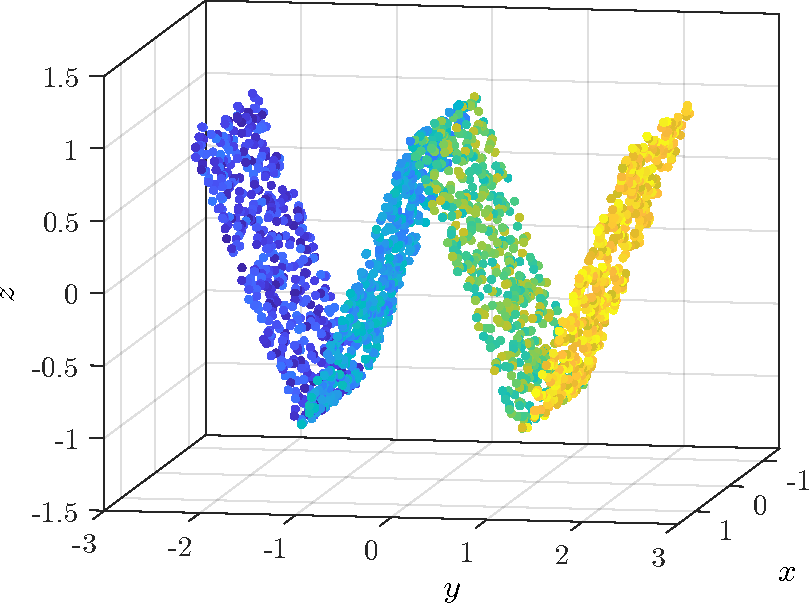
\includegraphics[width=8cm]{manifoldW.pdf}
    \caption{``W'' 形状流形数据分布图}
    \label{fig:manifoldW}
  \end{minipage}
  \begin{minipage}[t]{0.48\textwidth}
    \centering
    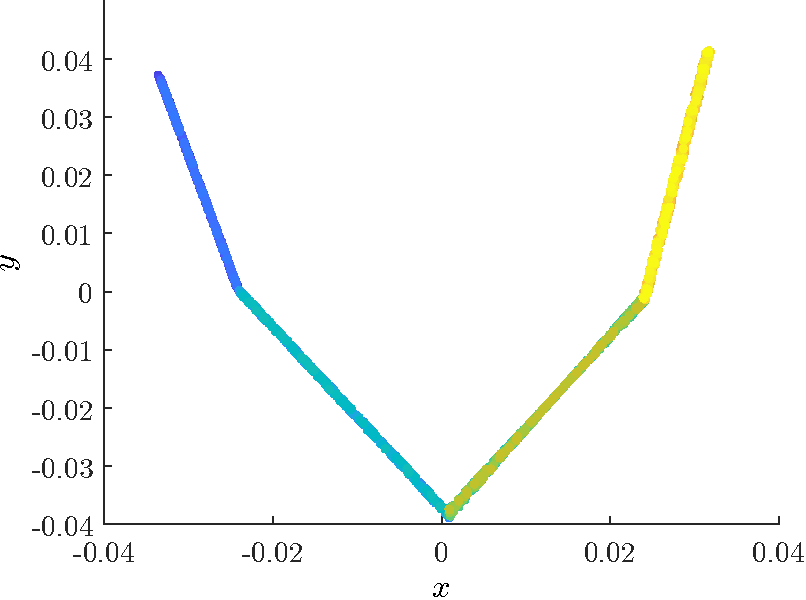
\includegraphics[width=8cm]{reducedW.pdf}
    \caption{``W'' 形状流形数据 40 近邻 LLE 降维结果}
    \label{fig:reducedW}
  \end{minipage}
\end{figure}

选择不同的近邻参数进行实验, 当近邻参数 $k$ 较小时, 降维结果均为与图 \ref{fig:reducedW} 类似的四条线段组成的折线, 而当近邻参数 $k$ 约等于一个平面的点数时, 降维结果为四个平行四边形组成的平面图形. ``W'' 的四个面均由 500 个点构成, 若取 500 近邻, 则 LLE 降维结果如图 \ref{fig:reducedW500} 所示, 此时 LLE 将三维数据降维到二维平面, 并且保持着数据点在二维流形上的位置关系.

\begin{figure}[htbp]
  \centering
  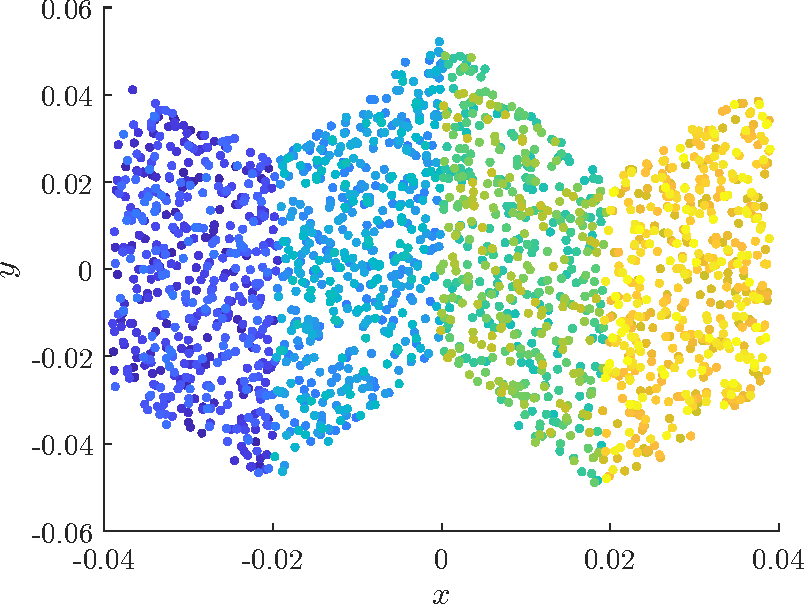
\includegraphics[width=10cm]{reducedW500.pdf}
  \caption{``W'' 形状流形数据 500 近邻 LLE 降维结果}
  \label{fig:reducedW500}
\end{figure}

\section*{Further Reading}

\subsection*{Whitening with PCA and ZCA}

``\emph{A whitening transformation or sphering transformation is a linear transformation that transforms a vector of random variables with a known covariance matrix into a set of new variables whose covariance is the identity matrix, meaning that they are uncorrelated and each have variance 1. The transformation is called `whitening' because it changes the input vector into a white noise vector.}'' \cite{whitening}

Suppose we have $n$ $d$-dimensional data points stored in $\vx \in \reals^{n \times d}$. The covariance matrix is $C(\bm{X}) = \frac{1}{n} \bm{X}^{T} \bm{X}$ and a whitening transformation is $\bm{Y} = \bm{W} \bm{X}$ where $\bm{W} \in \reals^{d \times d}$ is the whitening matrix and $\bm{Y}$ is the transformed data with $C(\bm{Y}) = \bm{I}$. Theoretically, whitening transformation is not unique because a rotated whitening matrix $\bm{W}_2 = \bm{R} \bm{W}_1$ ($\bm{R}$ is an orthogonal matrix) is also a whitening matrix. 

Suppose the eigenvalue decomposition for $C(\bm{X})$ is given by $C(\bm{X}) = \bm{E} \bm{D} \bm{E}^\top$ with eigenvectors in columns of $\bm{E}$ and eigenvalues on the diagonal of $\bm{D}$. For principal component analysis (PCA), the whitening matrix is calculated by $\bm{W}_{\text{PCA}} = \bm{D}^{-\frac{1}{2}} \bm{E}^\top$. For zero-phase component analysis (ZCA), the whitening matrix is $\bm{W}_{\text{ZCA}} = \bm{E} \bm{D}^{-\frac{1}{2}} \bm{E}^\top$. Multiplication by an orthogonal matrix can be seen as rotation and multiplication by a diagonal matrix can be seen as scaling. We can see that ZCA rotates the transformed vectors of PCA back to the original data space with the orthogonal matrix $\bm{E}$.

In deep learning, we know that batch normalization (BN) is a powerful trick to accelerate and stabilize the training of deep models. BN simply performs standardization for input feature maps. However, it has been shown that batch whitening (transform the input feature maps with a whitening transformation) further improves BN's optimization efficiency and generalization ability \cite{batch_whitening}. In batch whitening, the ZCA whitening is much better than the PCA whitening, read the work \cite{batch_whitening} for further reference of why this happens.

\emph{Optional:} Construct a toy example, calculate the PCA results and the ZCA results and compare them to illustrate why ZCA is preferred.


\subsection*{Non-classical MDS}

The classical derivation of MDS in the class assumed that the distance matrix is calculated by Euclidean distances of paired data points. However, in real applications, this matrix represents a set of dissimilarities which might not be Euclidean distances or not even distances at all. The MDS problem without the Euclidean assumption of distance matrix is called non-classical MDS. This is a generalization of the classical MDS and implemented as default MDS algorithm in Python library \href{https://scikit-learn.org/stable/modules/manifold.html#multidimensional-scaling}{scikit-learn}. Read the book \cite{MDS} for solutions in this situation.

In addition, there is a more general form of MDS algorithm called non-metric MDS which aims to preserve the \emph{rank-order} of the distances in the embedding space rather than their \emph{values}. You can also find solutions for non-metric MDS in the same book \cite{MDS} if you are interested.

% Reference
\begin{thebibliography}{1}

\bibitem{lle}

Sam T. Roweis, lle.m - A simple matlab routine to perform LLE, Locally Linear Embedding (LLE) Code Page, \url{https://cs.nyu.edu/~roweis/lle/code.html}.

\bibitem{whitening}
Wikipedia contributors. "Whitening transformation." Wikipedia, The Free Encyclopedia. Wikipedia, The Free Encyclopedia, 15 Dec. 2020. Web. 27 Apr. 2021. 

\bibitem{batch_whitening}
Huang L, Yang D, Lang B, et al. Decorrelated batch normalization [C]// Proceedings of the IEEE Conference on Computer Vision and Pattern Recognition. 2018: 791-800.

\bibitem{MDS}
Boyarski A., Bronstein A. Multidimensional Scaling. In: Ikeuchi K. (eds) Computer Vision. Springer, Cham, 2020.

\end{thebibliography}

\end{document}
